\chapter{Joshua 14}

\begin{figure}
  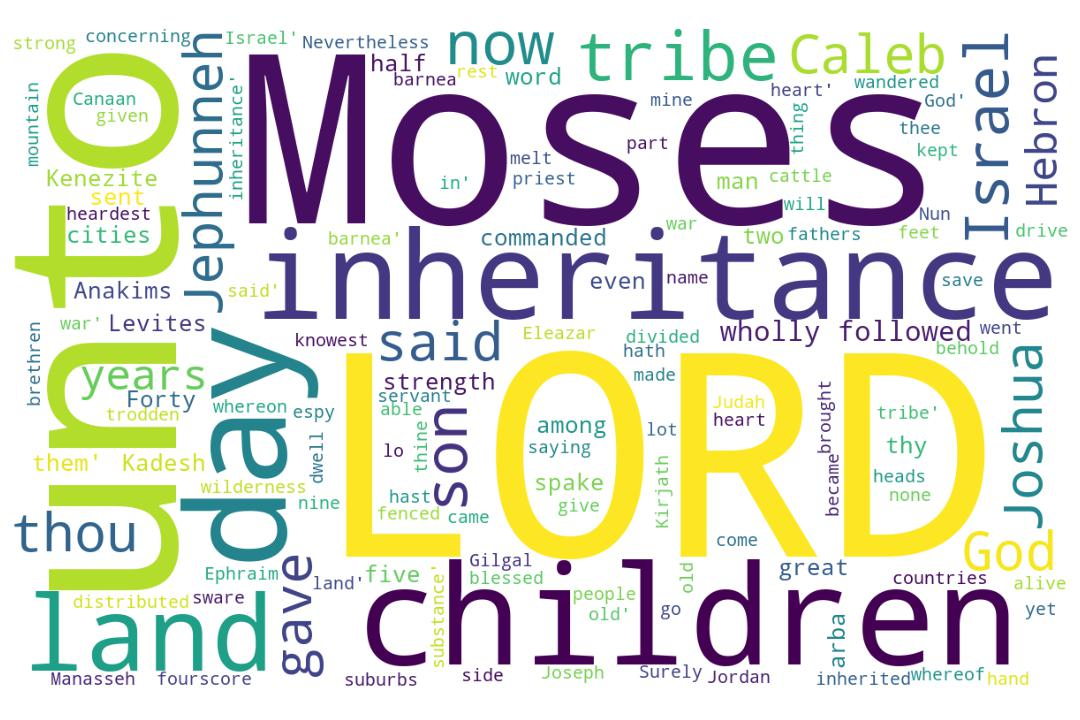
\includegraphics[width=\linewidth]{06OT-Joshua/Joshua14-WordCloud.jpg}
  \caption{Joshua 14 Word Cloud}
  \label{fig:Joshua 14 Word Cloud}
\end{figure}

\marginpar{\scriptsize \centering \fcolorbox{bone}{lime}{\textbf{CALEB'S VEIW}}\\ (Joshua 14) \begin{compactenum}[I.][8]
	\item \textbf{Countries Inherited}  \index[scripture]{Joshua!Jsh 14:01} (Jsh 14:1) 
	\item \textbf{Commands Heeded}  \index[scripture]{Joshua!Jsh 14:05} (Jsh 14:5) 
	\item \textbf{Caleb's Heart}  \index[scripture]{Joshua!Jsh 14:07} (Jsh 14:7) 
	\item A \textbf{Conspicuous Heritage}  \index[scripture]{Joshua!Jsh 14:09} (Jsh 14:9) 
	\item \textbf{Condemned Houses}  \index[scripture]{Joshua!Jsh 14:10} (Jsh 14:10) 
	\item \textbf{Courageous and Healthy}  \index[scripture]{Joshua!Jsh 14:11} (Jsh 14:11) 
\end{compactenum}}




\footnote{\textcolor[rgb]{0.00,0.25,0.00}{\hyperlink{TOC}{Return to end of Table of Contents.}}}\footnote{\href{https://audiobible.com/bible/joshua_14.html}{\textcolor[cmyk]{0.99998,1,0,0}{Joshua 14 Audio}}}\textcolor[cmyk]{0.99998,1,0,0}{And these \emph{are} \emph{the} \fcolorbox{bone}{lime}{\emph{countries}} which the children of Israel inherited in the land of Canaan, which Eleazar the priest, and Joshua the son of Nun, and the heads of the fathers of the tribes of the children of Israel, distributed for inheritance to them.}
[2] \textcolor[cmyk]{0.99998,1,0,0}{By lot \emph{was} their inheritance, as the LORD commanded by the hand of Moses, for the nine tribes, and \emph{for} the half tribe.}
[3] \textcolor[cmyk]{0.99998,1,0,0}{For Moses had given the inheritance of two tribes and an half tribe on the other side Jordan: but unto the Levites he gave none inheritance among them.}
[4] \textcolor[cmyk]{0.99998,1,0,0}{For the children of Joseph were two tribes, Manasseh and Ephraim: therefore they gave no part unto the Levites in the land, save cities to dwell \emph{in}, with their suburbs for their cattle and for their substance.}
[5] \textcolor[cmyk]{0.99998,1,0,0}{As the LORD \fcolorbox{bone}{lime}{commanded} Moses, so the children of Israel did, and they divided the land.}\\
\\
\P \textcolor[cmyk]{0.99998,1,0,0}{Then the children of Judah came unto Joshua in Gilgal: and Caleb the son of Jephunneh the Kenezite said unto him, Thou knowest the thing that the LORD said unto Moses the man of God concerning me and thee in \fcolorbox{bone}{MYGOLD}{Kadesh-barnea}.}
[7] \textcolor[cmyk]{0.99998,1,0,0}{Forty years old \emph{was} I when Moses the servant of the LORD sent me from \fcolorbox{bone}{MYGOLD}{Kadesh-barnea} to espy out the land; and I brought him word again as \emph{it} \emph{was} in \fcolorbox{bone}{lime}{mine heart}.}
[8] \textcolor[cmyk]{0.99998,1,0,0}{Nevertheless my brethren that went up with me made the heart of the people melt: but I wholly followed the LORD my God.}
[9] \textcolor[cmyk]{0.99998,1,0,0}{And Moses sware on that day, saying, Surely the land whereon thy feet have trodden shall be thine \fcolorbox{bone}{lime}{inheritance}, and thy children's for ever, because thou hast wholly followed the LORD my God.}
[10] \textcolor[cmyk]{0.99998,1,0,0}{And now, behold, the LORD hath kept me alive, as he said, these \fcolorbox{bone}{lime}{forty and five years}, even since the LORD spake this word unto Moses, while \emph{the} \emph{children} \emph{of} Israel wandered in the wilderness: and now, lo, I \emph{am} this day fourscore and five years old.}
[11] \textcolor[cmyk]{0.99998,1,0,0}{As yet I \emph{am} \emph{as} strong this day as \emph{I} \emph{was} in the day that Moses sent me: as my strength \emph{was} then, even so \emph{is} my \fcolorbox{bone}{lime}{strength} now, for war, both to go out, and to come in.}
[12] \textcolor[cmyk]{0.99998,1,0,0}{Now therefore give me this mountain, whereof the LORD spake in that day; for thou heardest in that day how the Anakims \emph{were} there, and \emph{that} the cities \emph{were} great \emph{and} fenced: if so be the LORD \emph{will} \emph{be} with me, then I shall be able to drive them out, as the LORD said.}
[13] \textcolor[cmyk]{0.99998,1,0,0}{And Joshua blessed him, and gave unto Caleb the son of Jephunneh Hebron for an inheritance.}
[14] \textcolor[cmyk]{0.99998,1,0,0}{Hebron therefore became the inheritance of Caleb the son of Jephunneh the Kenezite unto this day, because that he wholly followed the LORD God of Israel.}
[15] \textcolor[cmyk]{0.99998,1,0,0}{And the name of Hebron before \emph{was} Kirjath-arba; \emph{which} \emph{Arba} \emph{was} a great man among the Anakims. And the land had rest from war.}